\chapter{First- and second-order shallow flow modelling for flood simulation on heterogeneous computing devices}
\label{chapter:NumericalMethods}

The research presented herein leverages a first- and second-order finite-volume solution for the shallow water equations, as discussed and compared in the previous chapter. This chapter describes the mathematical background behind these numerical schemes, and a review of the background behind the methods selected. The numerical schemes can be considered a compromise between accuracy against analytical solutions, scope for efficient computation, and suitability for the hydrodynamics encountered in flooding from fluvial, pluvial, tidal, estuarine sources, and dam or defence failure scenarios. How these numerical methods lend themselves to high-performance computing architectures is then discussed, and the implementation details of the software framework provided.

\section{Numerical methods for shallow flows}

In the general case for a flood event, the water depth is much smaller than the horizontal dimensions of the water body. Therefore the hydrodynamics of the flood wave can be suitably described by the shallow water equations (SWEs) that are derived to take full account of mass and momentum conservation in a two-dimensional manner.

\subsection{Shallow water equations}

In matrix form, the SWEs may be written as

\begin{equation}
	\label{SWE_1stO}
	\frac{\partial\textbf{u}}{\partial t} +
	\frac{\partial\textbf{f}}{\partial x} +
	\frac{\partial\textbf{g}}{\partial y} =
	\textbf{s} ,
\end{equation}
where $t$ is the time, $x$ and $y$ the Cartesian coordinates, $\textbf{u}$ the vector representing the flow variables, $\textbf{f}$ and $\textbf{g}$ the fluxes in the two Cartesian directions, and $\textbf{s}$ is the source term vector. The vector terms are given by \citet{Liang2009b},

\renewcommand{\arraystretch}{1.5}
\begin{equation}
	\label{SWETerms_1stO}
	\begin{alignedat}{4}
		&\textbf u && = \left[ \begin{array}{c}
			\eta \\
			q_x \\
			q_y
		\end{array} \right] , \hspace{4ex} &
		&\textbf f &&  = \left[ \begin{array}{c}
			q_x \\
			uq_x + g(\eta^2 - 2\eta z_b)/2 \\
			uq_y
		\end{array} \right] ,\\
		&\textbf g && = \left[ \begin{array}{c}
			q_y \\
 			vq_x \\
			vq_y + g(\eta^2 - 2\eta z_b)/2 \\
		\end{array} \right] , \hspace{4ex} &
		&\textbf s && = \left[ \begin{array}{c}
			q_s \\
			-\frac{\tau_bx}{\rho} - g\eta \frac{\partial z_b}{\partial x} \\
			-\frac{\tau_by}{\rho} - g\eta \frac{\partial z_b}{\partial y} \\
		\end{array} \right] .
	\end{alignedat}
\end{equation}

Herein, $\eta$ and $z_b$ denote water level and bed elevation above datum and therefore $h = \eta - z_b$ calculates the water depth; $u$ and $v$ are the two depth-averaged velocity components; $q_x (= uh)$ and $q_y (= vh)$ are the $x-$ and $y-$directional unit-width discharges; $g$ is the gravitational acceleration; $q_s$ includes source and sink terms as a result of rainfall and loss through drainage systems, etc.;  $\rho$ is the water density; $-\delta z_b / \delta x$ and $-\delta z_b / \delta y$ define the two bed slopes; $\tau _{bx}$ and $\tau _{by}$ are bed friction stresses calculated by
\begin{equation}
	\label{SWE_1stO_BedFriction}
	\tau _{bx} = \rho C_f u\sqrt{u^2 + v^2} 
	\hspace{4ex} \textrm{and} \hspace{4ex}
	\tau _{by} = \rho C_f v\sqrt{u^2 + v^2} 
	,
\end{equation}
where $C_f = gn^2 / h^{1/3}$ is the bed roughness coefficient with $n$ known to be the Manning coefficient.

In order to better capture complex flow hydrodynamics including hydraulic jump-like flow discontinuities, the above SWEs are numerically solved using a finite-volume Godunov-type scheme, which updates flow variables to the next time step using the following time-marching formula,
\begin{equation}
	\label{SWE_1stO_Update}
	\textbf{u}_{i,j}^{k+1} 
	=
	\textbf{u}_{i,j}^{k}
	- \Delta t
	\left (
		\frac{\textbf{f}_{i+1/2, j} - \textbf{f}_{i-1/2, j}}{\Delta x}
		+
		\frac{\textbf{g}_{i, j+1/2} - \textbf{g}_{i, j-1/2}}{\Delta y}
		-
		\textbf{s}_{i,j}
	\right )
	,
\end{equation}
where $k$ represents the time level; $i$ and $j$ indicate the cell indices; $\Delta t$, $\Delta x$ and $\Delta y$ are the time step, cell size in the $x-$ and $y-$directions, respectively. In order to update the flow variables to a new time step, the four flux vectors $(f_{i+1/2, j}, f_{i-1/2, j}, g_{i, j+1/2}, g_{i, j-1/2})$ and the source term vector $(s_{i, j})$ must be properly calculated.

In the context of a Godunov-type scheme, the interface fluxes are evaluated by solving local Riemann problems, e.g. $\textbf{f}_E = \textbf{F}(\textbf{q}_E^L, \textbf{q}_E^R)$, that are defined by the left and right Riemann states $\textbf{q}_E^L$ and $\textbf{q}_E^R$. In order to obtain the Riemann states, the values of flow variables must first be reconstructed on both sides of the cell interface under consideration. A first-order accurate scheme assumes piecewise distribution of the flow information and therefore the face values are essentially the same as those at the cell centres. Taking the eastern cell interface of cell $(i, j)$ as an example, the left face values of the flow variables and bed elevation are simply
\begin{equation}
	\label{SWE_1stO_FaceValues}
	\textbf{q}_{E}^{L} = \textbf{q}_{ic}
	\hspace{4ex} \textrm{and} \hspace{4ex}
	\tilde{z}_{bE}^{L} = z_{b i,j}
	.
\end{equation}
Subsequently, the associated face values of water depth and velocity components are given by
\begin{equation}
	\label{SWE_1stO_FaceValues_huv}
	\tilde{h}_{E}^{L} = \tilde{\eta}_{E}^{L} - \tilde{z}_{bE}^{L}, \\
	\tilde{u}_{E}^{L} = (\tilde{q}x)_{E}^{L} / \tilde{h}_{E}^{L},
	\hspace{4ex} \textrm{and} \hspace{4ex}	\\
	\tilde{v}_{E}^{L} = (\tilde{q}y)_{E}^{L} / \tilde{h}_{E}^{L}
	.
\end{equation}

The face values on the right-hand-side of the cell interface can be obtained in a similar way, which is actually equal to those at the centre of cell $(i + 1, j)$. Based on these face values, the Riemann states are derived after defining a single value of bed elevation across the cell interface, i.e.
\begin{equation}
	\label{SWE_1stO_BedElev}
	z_{bE} = max \left ( \tilde{z}_{bE}^{L}, \tilde{z}_{bE}^{R} \right )
	.
\end{equation}

The corresponding Riemann states are therefore reconstructed as
\begin{equation}
	\label{SWE_1stO_Reconstruction}
	h_{E}^{L} = max \left ( 0, \tilde{\eta}_{E}^{L} - \tilde{z}_{bE}^{L} \right ), \\
	\eta_{E}^{L} = h_{E}^{L} + z_{bE}, \\
	(q_{x})_{E}^{L} = (\tilde{u})_{E}^{L} h_{E}^{L},
	\hspace{1ex} \textrm{and} \hspace{1ex}	\\
	(q_{y})_{E}^{L} = (\tilde{v})_{E}^{L} h_{E}^{L}
	.
\end{equation}
Similarly, the Riemann states can be obtained at the right hand side of the cell interface.

In the current formulation of SWEs as given in Equation \ref{SWE_1stO} and \ref{SWETerms_1stO}, the water level instead of water depth is used as a flow variable. In a dry cell, the reconstructed water level is actually the ground level. If the ground level (i.e. the reconstructed `water level') is higher than the actual water level, spurious fluxes will be calculated which in turn breaks the so-called well-balanced property of the governing equations. Therefore, the difference between the actual and fake water levels must be identified and subtracted from the reconstructed bed elevation and water level \citep{Liang2010a}. Again taking the eastern interface of cell $(i, j)$ as an example, the level difference can be easily calculated by
\begin{equation}
	\label{SWE_1stO_BedShift}
	\Delta z = max \left ( 0, z_{bE} - \tilde{\eta}_{E}^{L} \right )
	,
\end{equation}
which is then used to modified the reconstructed bed elevation and water level as follows

\begin{equation}
	\label{SWE_1stO_ShiftedStates}
	z_{bE} \leftarrow z_{bE} - \Delta z, \\
	\eta_{E}^{L} \leftarrow \eta_{E}^{L} - \Delta z,
	\hspace{4ex} \textrm{and} \hspace{4ex}	\\
	\eta_{E}^{R} \leftarrow \eta_{E}^{R} - \Delta z
	.
\end{equation}

\subsection{HLLC solution to the Riemann problem}

These reconstructed Riemann states are employed to define local Riemann problems, which are then solved by the HLLC approximate Riemann solver, i.e. the Harten, Lax and van Leer solver with the contact wave restored \citep{Toro1994}. This provides fluxes across each of the interfaces. Whilst an exact solution is obtainable for the Riemann problem, the iterative nature of the exact solution is not conducive to expedient computation. The HLLC method is widely recognised as providing enough accuracy for mainstream applications, although comparison and debate between a range of approximate solvers continues in the literature. The suitability of this method for applications with wetting and drying is acknowledged by \citet{Liu2013}, along with the improvements in accuracy it provides over the HLL method, while still relatively expedient to solve on modern computational hardware. Results provided by \citet{Erduran2002} show clear benefits in many cases of HLLC over HLL, whilst also acknowledging the performance benefits over some alternative but more accurate schemes; it is in effect presented as a middle-of-the-road solution, which is practical to implement, with considerable accuracy, and only marginally more expensive than HLL to compute, and broad suitability for "all kinds of applications".

The HLLC solution structure is illustrated in Figure \ref{RiemannProblem}, where the star region is indicated between two waves or shocks. The restored rarefaction wave is indicated by $S*$; more computationally intensive methods including HLLD \citep{Mignone2009} and Roe \citep{Roe1981} introduce further waves within the fan and consequently may be less diffusive.

\begin{figure*}[tpb]
\centering
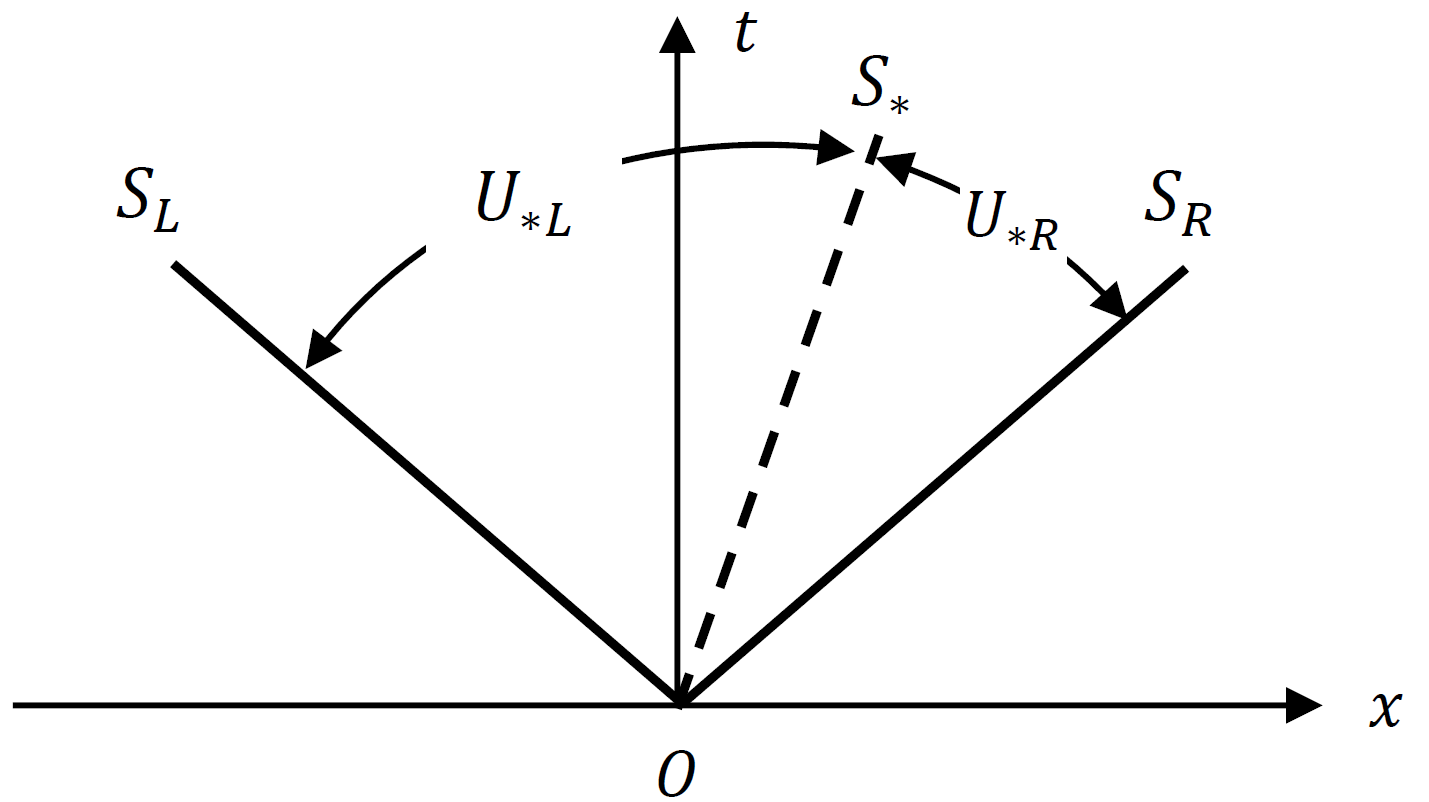
\includegraphics[width=0.75\textwidth]{numerical-scheme-figures/riemann-problem.png}
\caption{Diagrammatic representation of the approximate Riemann solution}
\label{RiemannProblem}
\end{figure*}

The full method is widely available, and is implemented exactly as described in \citet{Toro1994}, thus omitted here.

\subsection{Boundary conditions}

The extremities of the computational domain lack sufficient data to compute the numerical scheme, lacking neighbours on one or more faces. A variety of methods are available for the treatment of boundary conditions, it is far preferable numerically if the area of interest is sufficiently distant from the boundary, thereby reducing the influence of the method employed. The simplest approach is to prevent computation at the extremities and ensure these cells are dry; this is analogous to a waterfall in the real world, where flow is prohibited from returning. The Riemann solution across the interface is likely however to draw an excessive amount of water from upstream, which risks skewing nearby results.

For simulations where water must be contained within the domain, options are to reverse the flow direction and directly reflect flows, or create a wall using a high bed elevation which should also reflect flows albeit with some losses. The latter may prove more diffusive, but such an effect would also be expected in reality.

Boundary conditions describing river flows (i.e. a timeseries depth and discharge or velocity values) can either be introduced through the source term vector $\mathbf{s}$, or through careful manipulation of the cell states outside the numerical scheme. 

\subsection{Stability criterion}

The maximum permissible timestep for stability in the scheme is governed by the work of Courant-Friedrichs-Lewy \citep{Courant1967}, or the so-called CFL condition
\begin{equation}
	\label{CFL}
	\Delta t = C \cdot min \left[\frac{\Delta x}{\lvert u + \sqrt{gh} \rvert} , \frac{\Delta y}{\lvert v + \sqrt{gh} \rvert}\right] ,
\end{equation}
where \(C\) is the Courant number, with constraint \(0 < C \le 1\). The CFL condition is applied to all of effective computational cells, and the largest permissible time step is thereby used to advance the numerical scheme to the next time increment. It is worth noting the limitations of this approach, insofar as $\sqrt{gh}$ describes the phase velocity of shallow water waves, but the shallow water model presented herein will be applied across a range of scenarios. Shocks and discontinuities not fully addressed by Equation \ref{CFL} also become more likely at high grid resolutions, hence values of $C$ are typically kept below $0.7$ for the work herein, consistent with the findings of \citep{Erduran2002}. A halving in the grid size will result in a four-times increase in the number of cells, whilst also halving the CFL-constrained timestep, thus typically increasing simulation workload eight-fold.

\subsection{Source terms for energy loss and topographic slope}
\label{sec:source-terms}

The bed slope source terms are directly approximated by a central differencing approach. For example, in the $x$-direction,

\begin{equation}
	\label{SWE_1stO_BedSlope}
	-g \eta \frac{ \delta z_b }{ \delta x } = -g \tilde{\eta} \left ( \frac{ z_{bE} - z_{bW} }{ \Delta x } \right )
	,
\end{equation}

where $ \tilde{\eta} = ( \eta_{E}^{L} + \eta_{E}^{R} )^2 $. 

For the friction source terms, a splitting-limited-implicit scheme adopted by \citet{Liang2010a} is implemented to ensure better numerical stability. This gives a robust finite-volume Godunov-type solver for simulating shallow flows over complex domain topography with wetting and drying. The point-implicit scheme is given through Taylor expansion of an ordinary differential equation accounting for friction effects. This approach allows for a solution which is independent of the Godunov-type scheme. Neglecting higher-order terms in the expansion, unit-width discharges after accounting for friction become
\begin{equation}
	\label{Friction}
	\begin{alignedat}{3}
		&q_{x}^{t+\Delta t} && = q_{x}^{t} + \Delta tF_x && ,\\
		&q_{y}^{t+\Delta t} && = q_{y}^{t} + \Delta tF_y && ,\\
	\end{alignedat}
\end{equation}
where for axis \(x\) and perpendicular axis \(y\),
\begin{equation}
	\label{FrictionPrereq}
	\begin{alignedat}{2}
		&F_x      && = \frac{S_{fx}}{D_{dx}} ,\\
		&S_{fx}   && = -q_x\frac{C_f}{h^2}\sqrt{q_{x}^{2} + q_{y}^{2}} ,\\
		&D_{dx}   && = 1 + \Delta t \times \frac{C_f}{h^2} \times \frac{2q_x + q_y}{\sqrt{q_{x}^{2} + q_{y}^{2}}} ,\\
		&C_f      && = \frac{gn^2}{h^{\frac{1}{3}}} .
	\end{alignedat}
\end{equation}

\section{Extension to second-order solution}

A MUSCL-Hancock approach \citep{VanLeer1984} is adopted to achieve second-order accuracy in both space and time. Specifically, cell face-extrapolated values are obtained using a MUSCL linear reconstruction method implemented with a MINMOD slope limiter \citep{Roe1986} for flow variables \(\begin{matrix}[\eta & uh & vh]\end{matrix}^T\) to prevent spurious oscillations that might otherwise be introduced \citep{Toro2001}. This ensures the scheme is total variation diminishing (TVD). The MINMOD limiter is selected herein because its properties provide better numerical stability for a wide range of conditions \citep{Suresh2000,Yee2006}, and while it is also diffusive by way of comparison to alternative methods, the advantages in terms of stability were considered superior.

These choices were guided by \citet{Erduran2002}, where the authors conclude second-order accuracy is sufficient for almost all cases, including large discontinuities, and acknowledge that in practical applications stability may be compromised with Courant numbers exceeding $0.7$.

A half-timestep evolution of the cell states is introduced for each iteration, using slope-limited values extrapolated towards each of the cell interfaces. Considering each of the primitive variables composing $\textbf{u}$ in Equation \ref{SWE_1stO} piece-wise as $u$, along an axis, the slope ratio for a cell is computed as 
\begin{equation}
	\label{SWE_SlopeRatio}
	r_i = \frac{u_i - u_{i-1}}{u_{i+1} - u_i}
	.
\end{equation}
Each slope ratio is limited using the MINMOD function given by \citet{Toro2001}, which can be simplified for this application to give,
\begin{equation}
	\label{SlopeLimiter_MINMOD}
	\phi_{mm}(r) = max(0, min( 1, r_i ))
	.
\end{equation}
Piece-wise application of the slope functions, $\phi_{mm}(r)$, to the vector \(\begin{matrix}[\eta & h & uh & vh]\end{matrix}^T\) provides a slope vector $\mathbf{\bar{\Delta}}$, which is applied along each axis, giving two face-extrapolated vectors, $\mathbf{u}_i^L$ and $\mathbf{u}_i^R$ for each,
\begin{equation}
	\label{MUSCL_FaceExtrapolation}
	\mathbf{u}_i^L = \textbf{u}_i - \frac{1}{2}\mathbf{\bar{\Delta}}\hspace{4ex}, \\
	\mathbf{u}_i^R = \textbf{u}_i + \frac{1}{2}\mathbf{\bar{\Delta}}\hspace{4ex}
	.
\end{equation}

Application of the slope limiter along each axis provides a face-extrapolated vector for each Cartesian direction, \(\begin{matrix}u^N & u^E & u^S & u^W\end{matrix}\). These are used to advance the cell states by a half-timestep,
\begin{equation}
	\label{SWE_MUSCL_HalfTimestep}
	\begin{alignedat}{2}
	\mathbf{u}_{i,j}^{t+\Delta\frac{1}{2}} 
	=
	\mathbf{u}_{i,j}^{t}
	& - \frac{1}{2} \frac{\Delta t}{\Delta x} (\mathbf{f}(\mathbf{u}^E) - \mathbf{f}(\mathbf{u}^W)) \\
	& - \frac{1}{2} \frac{\Delta t}{\Delta y} (\mathbf{g}(\mathbf{u}^N) - \mathbf{g}(\mathbf{u}^S)) \\
	& + \frac{1}{2} \Delta t \mathbf{s} 
	\hspace{4ex},
	\end{alignedat}
\end{equation}
using modified functions to evaluate the flux, where the bed elevation is derived from the face-extrapolated vectors, as for $\mathbf{f}$ and $\mathbf{g}$ in Equation \ref{SWETerms_1stO}.

Friction terms can be omitted from the source terms at this point, and later applied using the point-implicit scheme in Section \ref{sec:source-terms}. The half-timestep advanced cell states are extrapolated using the same piece-wise application of slopes in Equation \ref{MUSCL_FaceExtrapolation} and carried forward for use evaluating the full-timestep with Riemann solutions.

The methods employed herein provide a second-order accurate solution under normal circumstances, but will fall back to a first-order solution at the wet-dry interface. The limiter function is constrained so as to ensure the solution remains within the TVD region. Research remains ongoing with regard to the treatment of wet-dry interfaces, avoidance of spurious velocity measurements, and maintaining numerical stability with high-order methods, such as in the work of \citet{Hou2013}.

\section{Solution using heterogeneous architectures}

The equations and methods described in this chapter thus far, given their iterative, time-marching and piece-wise nature, require the assistance of computers to be applied. The approximately eight-fold increase in computational expense for each halving of the grid resolution is problematic for application at high resolutions, in dense urban environments, and so prudence and considered software design is required to make these simulations feasible. As previously discussed, many computers offer either hybrid processor architectures, or more than one form of processor with different intended applications, most notably general computational and graphic rendering. The remainder of this chapter focuses on the software design approach required to map the numerical scheme to these processors, in an efficient manner.

\begin{figure*}[bp]
	\centering
	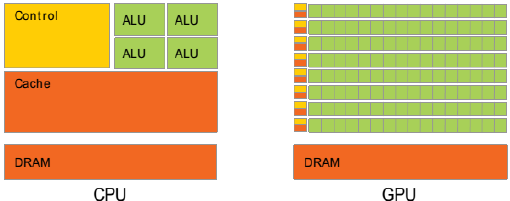
\includegraphics[width=0.7\textwidth]{numerical-scheme-figures/cpu-gpu-architecture.png}
	\caption{A simplified comparison of the differences between CPU and GPU architectures.}
	\label{CPUGPUArchitecture}
\end{figure*}

The GPU is so-named because its design and purpose is to accelerate graphics calculations, primarily 3D rendering such as in computer games. The calculations are performed within `shaders', small program designed to perform a specialised set of matrix calculations with uniform values (e.g. the position of the sun to calculate shadows) and vectors. A vertex shader is executed over all the vertices that form the 3D model, to compute a 2D on-screen position from the 3D world, and a fragment shader subsequently over each of the pixels, to compute lighting effects and sample textures. A smooth experience requires a throughput of up to 90 frames per second, hence these processors are highly specialised; shader programs typically do not change during execution, and may be executed simultaneously on enormous volumes of data, such as for the $\gtrapprox 1.3M$ pixels on a typical computer screen.

A simplified comparison of the two processor architectures is shown in Figure \ref{CPUGPUArchitecture}, where the far higher ratio of arithmetic logic units to control units is seen; this is because a single controller can instruct many logic units to perform the same calculation. This architecture is known as single-instruction multiple-data (SIMD). Their performance is typically measured in terms of floating point operations per second (FLOPS), although the difference between theoretical maximum and the rate achievable in practice (where data must be read and written) is usually substantial.

\begin{table*}[pb]
	\newcolumntype{R}[1]{>{\RaggedLeft\arraybackslash}p{#1}}
	\small
	\centering
	\caption{Comparison of some of the CPU and GPU devices employed in this thesis, with prices correct in 2013.}
	\label{CPUGPUCosts}
	\begin{tabular}{p{0.3\textwidth}R{0.2\textwidth}R{0.2\textwidth}R{0.2\textwidth}}
		\hline
										& \textbf{CPU} Intel i7 950 3GHz & \textbf{GPU} AMD FirePro V7800 ($\times$2) & \textbf{GPU} NVIDIA Tesla M2075 ($\times$4) \\
		\hline
		Cost							& £260						& £1,200						& £10,000			\\
		64-bit FLOPS $\times10^{9}$		& 49						& 806							& 2,064				\\
		Device memory (GB)				& N/A						& 4.0 (2.0 $\times$ 2)			& 24.0 (6.0 $\times$ 4) \\
		Cost per FLOP $\times10^{9}$		& £5.20						& £1.49							& £4.84				\\
		\hline
	\end{tabular}
\end{table*}

The advantages of leveraging GPU devices become more apparent when the costs are examined. Table \ref{CPUGPUCosts} outlines the cost per unit of computing power for some of the devices used herein, which for these cases are all capable of residing within a single computer (division of work across devices in more than one computer is discussed later). The GPU devices, whilst less versatile, provide more power per pound expended, although it is worth noting a GPU device cannot operate without a counterpart CPU, and most likely at least the same memory available to the CPU as GPU. The M2075 GPU represents a professional-grade device targeted at general-purpose computation rather than graphics, hence the greater cost.

\subsection{Control flow and software structure}

The Open Computing Language (OpenCL) is a consortium-led project involving multiple hardware vendors that allows developers to produce low-level code compatible with a variety of modern CPUs, GPUs and APUs (a hybrid-style processor allowing some of both benefits on a single chip) available from NVIDIA, AMD and Intel \citep{KhronosOpenCLWorkingGroup2012,NVIDIACorporation2010,AdvancedMicroDevicesInc2011}. The software developed herein uses OpenCL to provide the greatest compatibility between different device and hardware configurations, whilst the performance levels achievable are comparable to popular alternatives such as CUDA \citep{Fang2011}. Non-parallelised parts of the software were developed in C++. Differences in architecture, quantity of, and structure of compute units (which may be a core for a CPU, or a streaming multiprocessor for a GPU, depending on the manufacturer and architecture), and memories available thereon make it difficult to design code which can be considered optimised across a large number of devices. A new model structure is presented in this work to cope with these difficulties, and variations in memory management are assessed to determine their effect.

Successful and efficient implementation for GPUs requires careful consideration of the six elements shown in Figure \ref{ModelComponents}, where a kernel refers to a discrete function within the program that can be executed in parallel across a range of data, and a reduction entails identifying a single value (e.g. minimum, maximum, or sum) from a large number of elements. To address hardware differences properly, the software developed allows end-user configuration of floating-point precision, workload balance in data reductions, and caching from global to local memory where applicable. Unlike existing software, a suitable and optimised configuration should therefore be achievable for any device conformant to the OpenCL specification.

A regular Cartesian grid of \(M \times N\) cells is used. This reduces the total data requirement and computational burden as no structure is necessary relating cells, and trigonometric functions are not required to update cells. Static cell data and initial conditions for transient variables are read from raster files using the Geospatial Data Abstraction Library (GDAL), thereby providing support for most common GIS file formats. Device-specific binaries are compiled before each simulation with the system's OpenCL drivers, allowing pre-processor macros to define many constants including the domain dimensions. 

Code responsible for applying the finite-volume scheme is generated at least in part dynamically, then compiled by the underlying operating system drivers using an appropriate instruction set and optimisations for the hardware available, a process which typically takes $<1$ second. This is accomplished through the Application Programming Interface (API) functionality made available through the OpenCL standard. Relevant constants such as the cell dimensions of the domain are hence embedded in the assembly instructions themselves, and functionality which is not required or disabled (e.g. friction, atmospheric boundary conditions) can be removed altogether. Dynamic type definitions also allow the same codebase to be used with single- (32-bit) or double-precision (64-bit) floating-point arithmetic, which refers to the memory allocated to storing the significand and exponent to represent decimal numbers, in the manner employed by almost all modern computers, per IEEE 754 \citep{InternationalOrganizationforStandardization2011}.

A small overhead is associated with executing kernels and receiving notification of completion with blocking commands or callbacks. This is alleviated by adding multiple iterations of the numerical scheme to the execution queue and only displaying progress feedback periodically. Consequently, kernels are occasionally queued unnecessarily, as the simulation cannot progress further until output files are written; in such cases the timestep reduces to zero and kernels will exit early. The main loops operating on the compute device and host computer to coordinate this are shown in Figure \ref{HiPIMS_Structure_NoVis}, where there will be numerous iterations of the OpenCL loop before returning to the host computer loop.

\begin{figure*}[tpb]
	\centering
	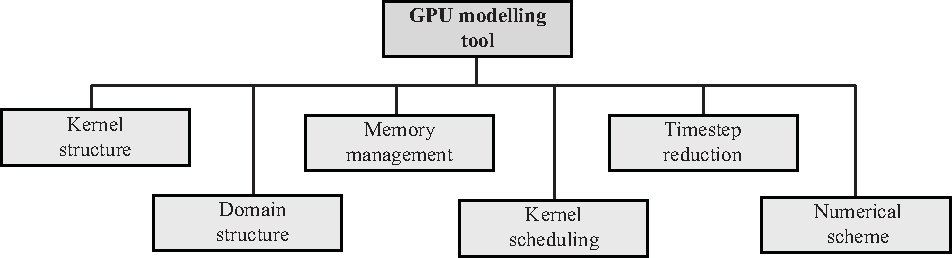
\includegraphics[width=0.95\textwidth]{heterogeneous-dev-figures/Figure_1_Greyscale.pdf}
	\caption{Main considerations for designing the shallow-flow modelling tool.}
	\label{ModelComponents}
\end{figure*}
\begin{figure*}[pb]
	\centering
	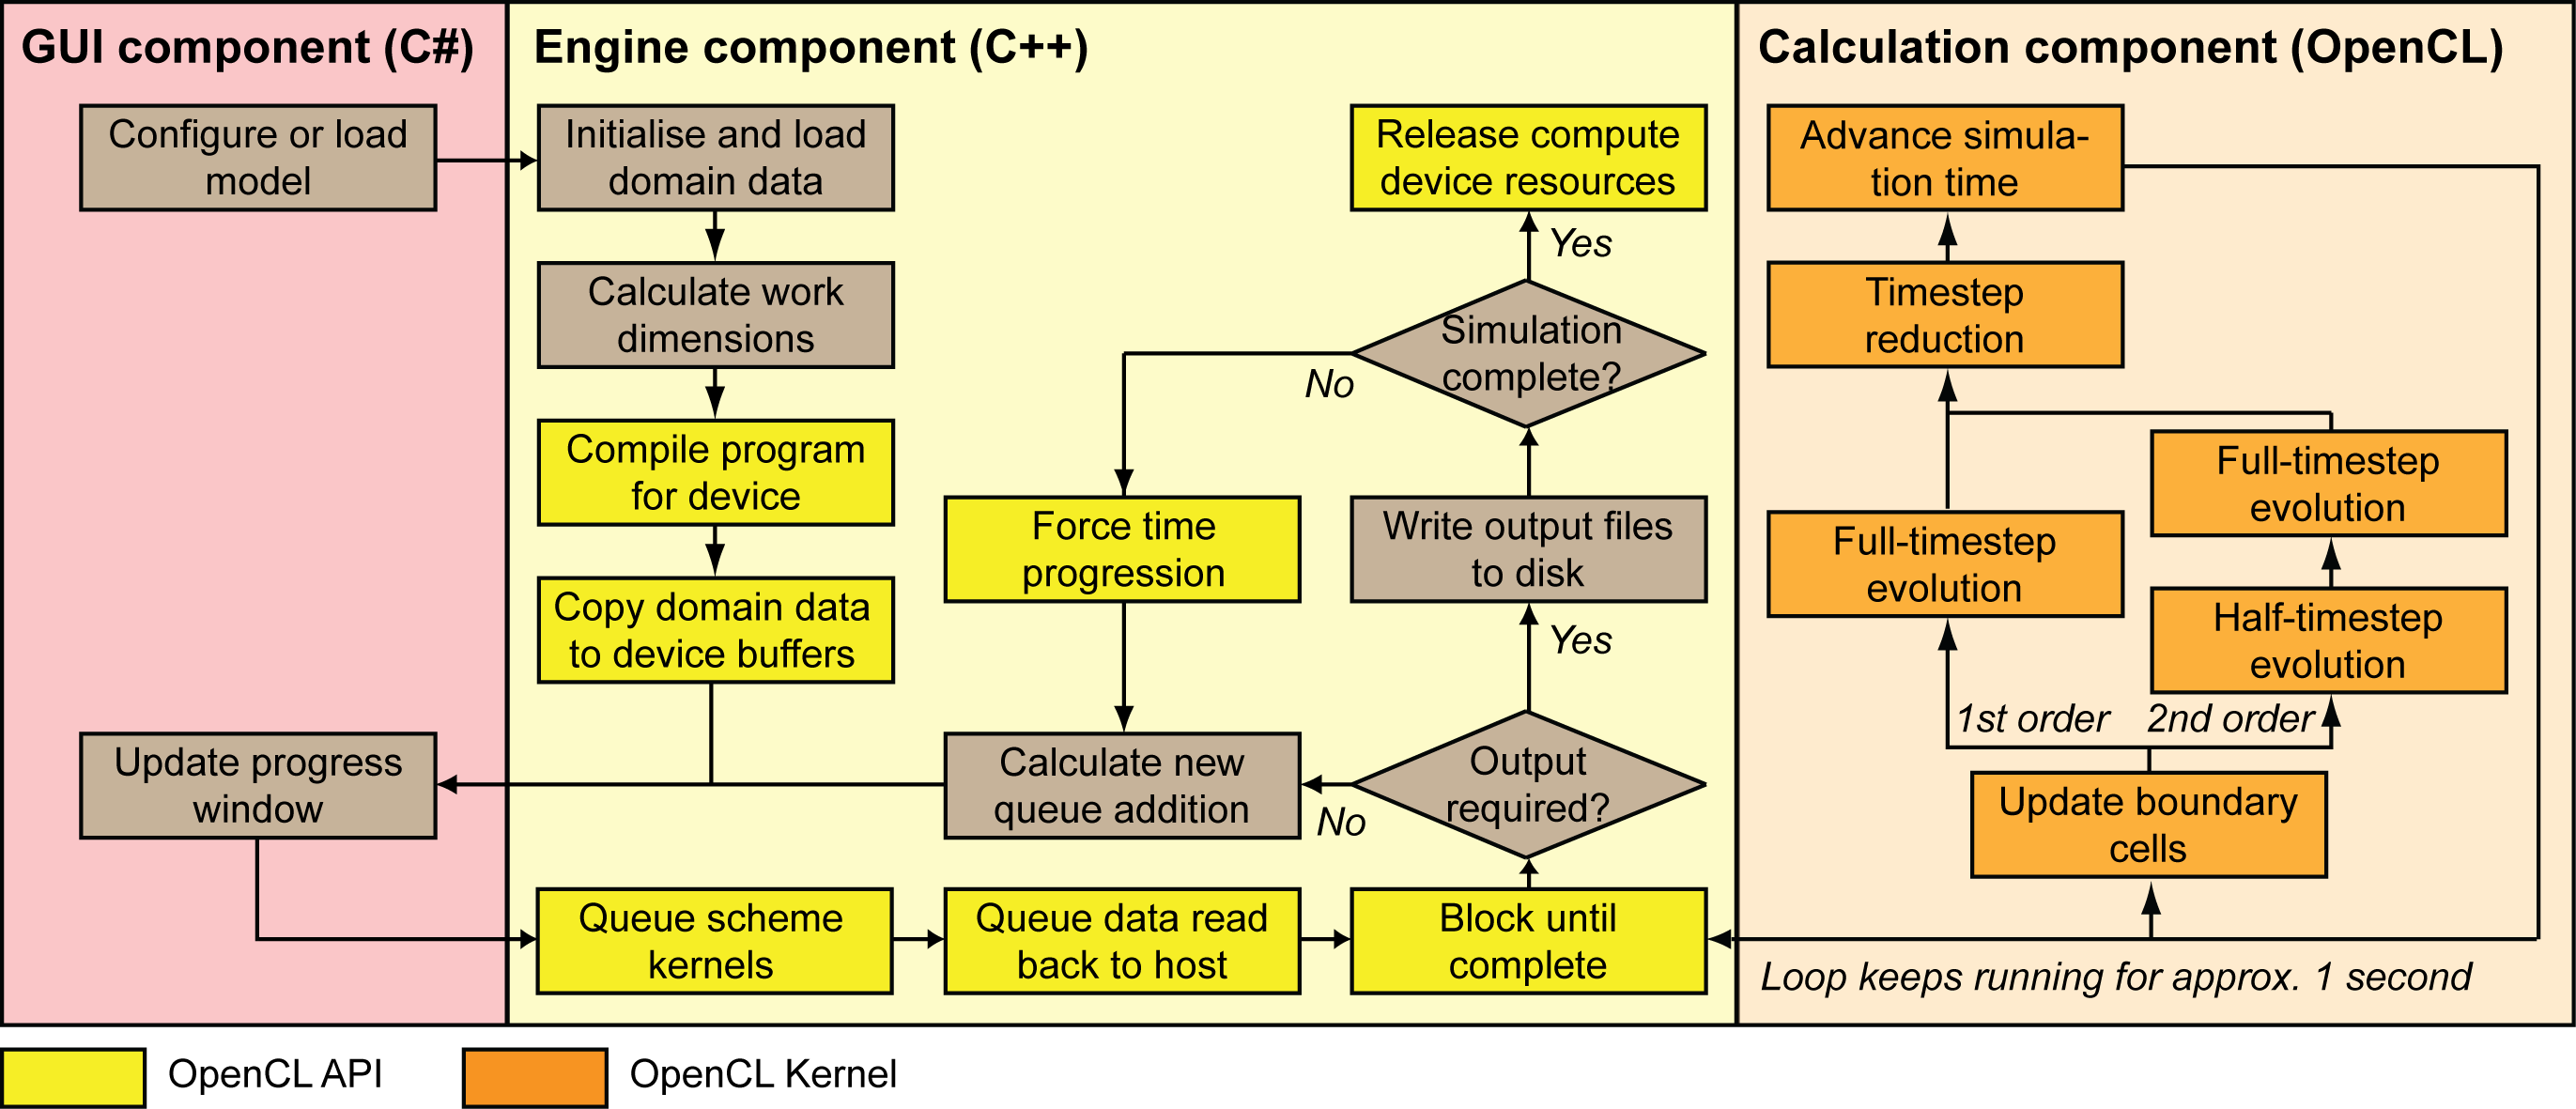
\includegraphics[width=1.0\textwidth]{heterogeneous-dev-figures/HiPIMS_Structure_NoVis.png}
	\caption{Flowchart of the software processes indicating which components are OpenCL kernels or API calls.}
	\label{HiPIMS_Structure_NoVis}
\end{figure*}

Moving data from the main system memory (RAM) to a GPU device is an expensive operation \citep[see recommendations in][]{AdvancedMicroDevicesInc2011,NVIDIACorporation2010a}. Cell data is only moved periodically for output files, and the numerical scheme is otherwise permitted to run in a loop for approximately one second before a small amount of data is transferred to update the user on the progress of the simulation. This process is represented in Figure \ref{HiPIMS_Structure_NoVis}. No vendor-specific optimisations were made, as the author's intention was to create a system appropriate for use with any of the mainstream vendors' hardware, most notably NVIDIA, AMD and Intel, but any conformant implementation of the OpenCL 1.2 standard should be capable of running the code. The compiler is instructed to adhere to all of the appropriate IEEE standards for floating-point arithmetic (i.e. accurate square root operations, treatment of denormals, etc.).

A regular Cartesian grid is used to represent the domain, whereby transient state variables are stored in a four-element vector and constant values (bed elevation and friction coefficients) require two further elements. This means 48 bytes or less are required per cell. Considering further constraints imposed on the size of a single memory allocation, the software is presently limited to $\approx$130 million cells for current hardware offering up to 16GB of memory.

A variety of raster formats are supported for importing and exporting domain data, initial conditions, and periodic output. 

\subsection{Identification of CFL-constrained timestep}

A two-stage reduction process is used to identify the largest permissible timestep within the domain: cells are sampled with a regular stride through the array of cells, followed by recursive binary comparisons used to provide a single value which is carried forward to a much smaller array, as shown in Figure \ref{HiPIMS_Reduction}. This is examined in the second stage when incrementing the overall simulation time. The reduction process ensures processors perform sufficient work to mask the considerable latency introduced by transferring data from a GPU's globally-accessible memory to compute unit-specific registers.

\begin{figure*}[tpb]
	\centering
	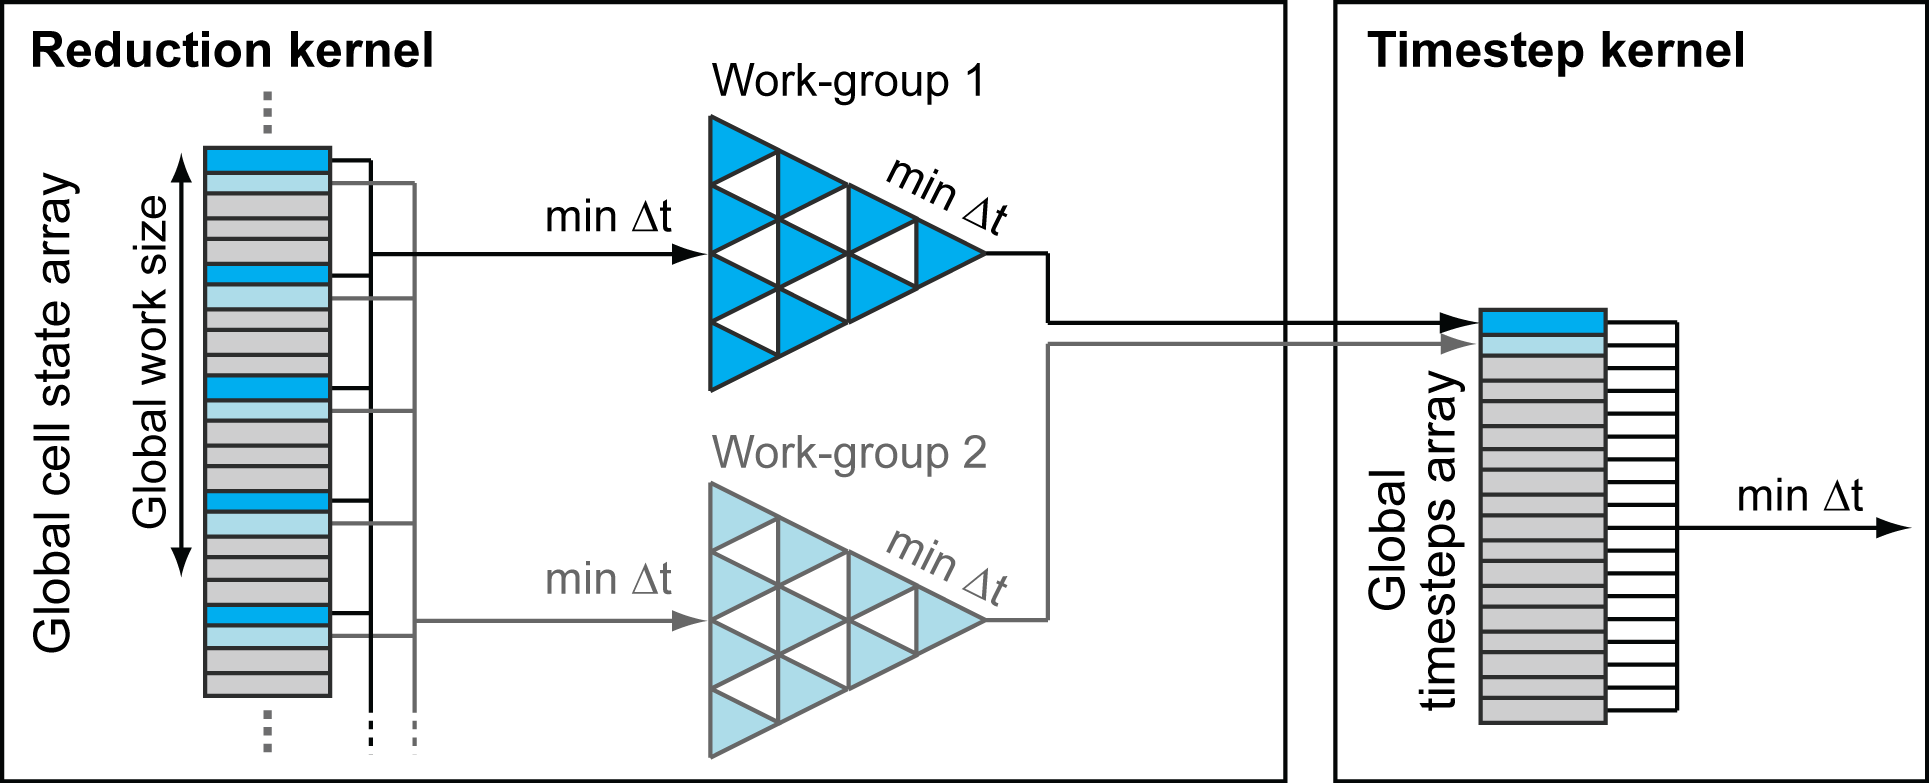
\includegraphics[width=0.8\textwidth]{heterogeneous-dev-figures/HiPIMS_Reduction_Colour.png}
	\caption{Representation of a two-stage reduction process with a global stride of six (stride in reality would be much larger) performing a series of binary comparisons to create a smaller array of potential values.}
	\label{HiPIMS_Reduction}
\end{figure*}

\subsection{Storage and memory access patterns in a heterogeneous environment}
\label{Subsection:StorageMemoryHeterogeneous}

The memory model adopted in OpenCL is composed of private (i.e. registers), local (or LDS), and global (including constant) memory; Figure \ref{OpenCLStructure} is a simplified representation of these memories. Global memory is the largest resource in which all data that persists throughout the simulation must reside. Scientific GPUs presently offer up to 16GB of global memory.

\begin{figure*}[tpb]
	\centering
	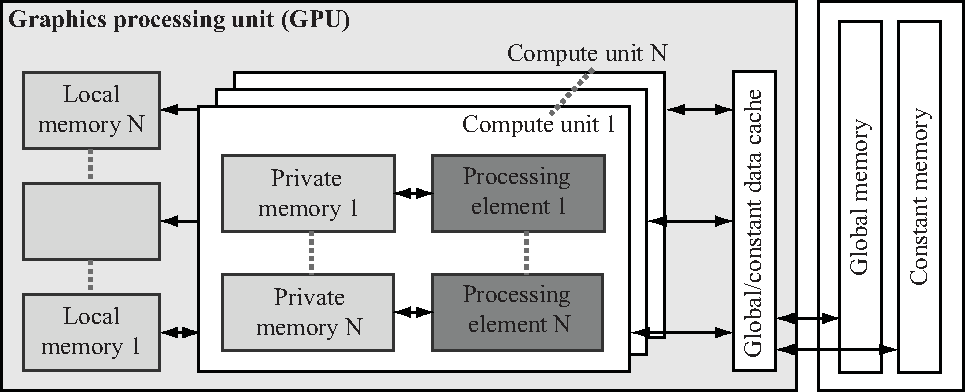
\includegraphics[width=0.8\textwidth]{heterogeneous-dev-figures/Figure_2_Greyscale.pdf}
	\caption{Memory model adopted in OpenCL, representing the structure of a GPU device and its global, local, private, and constant memory.}
	\label{OpenCLStructure}
\end{figure*}

The scheme used herein is directionally unsplit, thus both axes are considered simultaneously by kernels. A first-order solution is therefore dependent on data from four neighbouring cells, but a second-order solution is dependent on data from twelve cells, which as demonstrated in Figure \ref{RequisiteCellData} requires accessing global arrays using irregular strides. An alternative solution that reduces global accesses per cell is to commit cell data to local memory, synchronise the work-group, and subsequently access only that resource for neighbour data. 

\begin{figure*}[tpb]
	\centering
	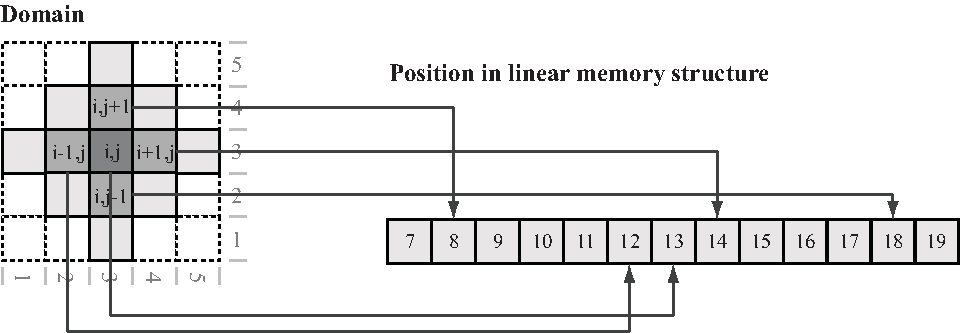
\includegraphics[width=1.0\textwidth]{heterogeneous-dev-figures/Figure_3_Greyscale.pdf}
	\caption{Requisite neighbour cell data to advance cell (i,j) demonstrating irregular strides when accessing global arrays, for a second-order solution.}
	\label{RequisiteCellData}
\end{figure*}

The minimum amount of local memory available for devices conformant to the OpenCL specification is 32kB, but maintaining activity on at least four work-groups requires each kernel to consume 8kB or less of local memory. Committing cell data for the whole work-group to local memory using a typical GPU work-group size of 256 hence allows for only 32 bytes of data per cell (i.e. four double-precision values).  This is insufficient to store four sets of cell face-extrapolated half-timestep advanced values. Moreover, cells towards the extremity of a work-group cannot be solved using the data in the local cache because neighbours are absent, so work-groups are required to overlap and the global work size is increased accordingly. Without caching, the whole work-group can be considered productive and no overlap is required. Caching for a prediction kernel requires a single layer overlap and increases the global work size by 30\% for a work-group size of 256, whereas caching for the whole computation in a single kernel is both arithmetically intensive and requires a double layer overlap, drastically increasing the global work size by 78\%. To address these constraints in this work, face-extrapolated data are held only in global or private memory depending on the configuration. Similarly, conserved variables may be configured as cached to local memory or read directly from global memory.

Finally, local memory on GPUs is divided into banks (typically 16 or 32); serialisation is required for accesses to addresses in the same bank (i.e. conflicts). These can be avoided by manipulating the dimensions of the cache array to introduce padding, but the increased memory consumption may reduce the number of schedulable units running simultaneously.

\subsection{Decomposition to stencil operations}

GPU architectures were designed and intended for graphical applications, especially rendering 3D objects in a 2D plane, as discussed earlier in this chapter. These operations are referred to as stencil operations, where the element under consideration is dependent only on constants (e.g. the position of the camera in 3D, or the timestep for fluids) and its neighbouring elements.

\begin{figure*}[tpb]
	\centering
	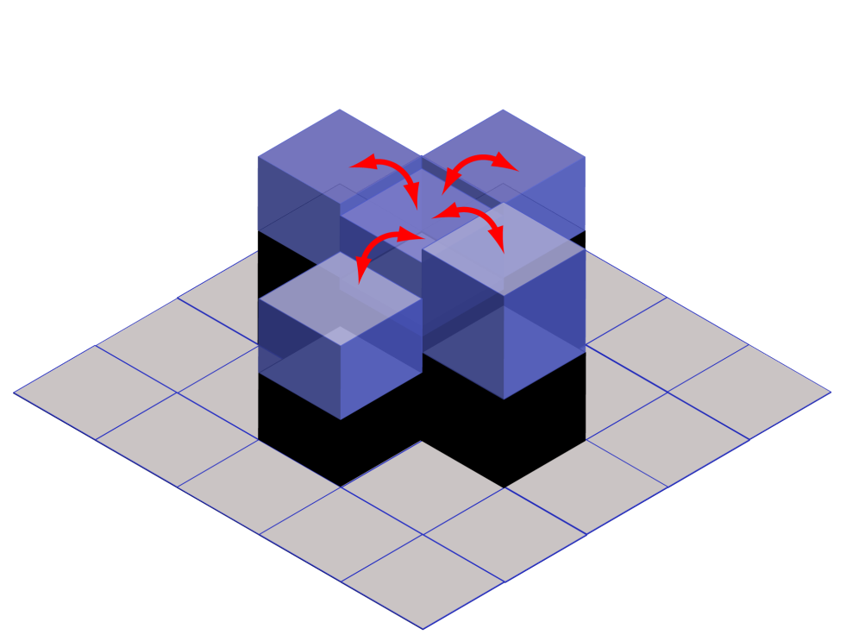
\includegraphics[width=0.95\textwidth]{heterogeneous-dev-figures/Stencil_Operation.png}
	\caption{Representation of the stencil operation with one cell dependent on its neighbours and fluxes between.}
	\label{StencilOperation}
\end{figure*}

Considering the first-order solution to the SWEs from earlier in the chapter, this can be expressed per Figure \ref{StencilOperation} as a series of stencil operations:
\begin{itemize}
	\item calculate fluxes between the cell of interest and each of its four neighbours;
	\item calculate the effect of those fluxes on discharge and free-surface level for the cell of interest, and apply the change.
\end{itemize}

The first-order solution with the HLLC method is dependent on four neighbouring cells; the data requirements are significant, and will affect computational performance.

The above method can be extended for the second-order solution, in which each neighbouring cell is also dependent on its neighbours. The overall data requirements increase accordingly to twelve neighbouring cells, but if the whole process is considered as two steps, the half- and full-timestep, then each step remains dependent on only four neighbouring cells with an additional requirement to store data between the two steps.

A kernel in OpenCL is executed over the global work (i.e. whole domain), within which there are work-groups of work-items, as shown in Figure \ref{OpenCLExecStructure}. A different work-item therefore handles each cell in the domain with reference to data held for neighbouring cells. For a GPU, work-groups are decomposed to schedulable units of wavefronts (so-termed by AMD, not to be confused with actual waves) or warps (NVIDIA) for execution; specifics and vendor differences can be found in \citet{KhronosOpenCLWorkingGroup2012,NVIDIACorporation2010,AdvancedMicroDevicesInc2011}. Each processing unit should be constantly engaged in productive computation to achieve the best performance with GPU architectures, known as the level of occupancy. It requires that each processing unit is assigned multiple schedulable units, allowing high-latency operations (e.g. global memory accesses, which are equivalent to hundreds of clock cycles \citep{NVIDIACorporation2010}) to be masked by the device's scheduling. Occupancy generally benefits from a high ratio of arithmetic operations to global data accesses but scheduling further units delivers no further benefit once a high occupancy is already achieved \citep{AdvancedMicroDevicesInc2011}. Consequently there is no panacea for optimisation on every device when transposing the numerical scheme to kernels.

\begin{figure*}[tpb]
	\centering
	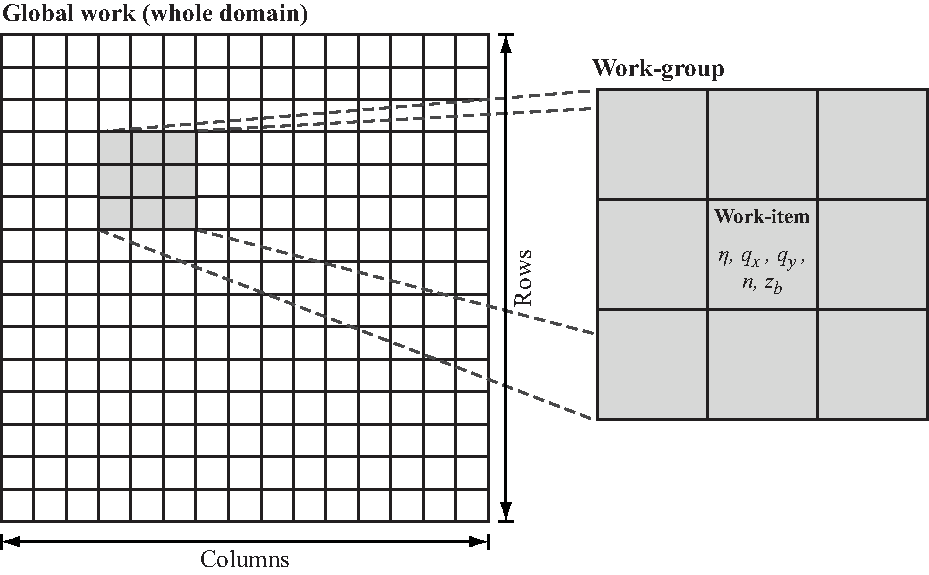
\includegraphics[width=1.0\textwidth]{heterogeneous-dev-figures/Figure_4_Greyscale.pdf}
	\caption{Structure of the OpenCL execution model as applied to the numerical scheme and domain structure herein.}
	\label{OpenCLExecStructure}
\end{figure*}
\begin{figure*}[tpb]
	\centering
	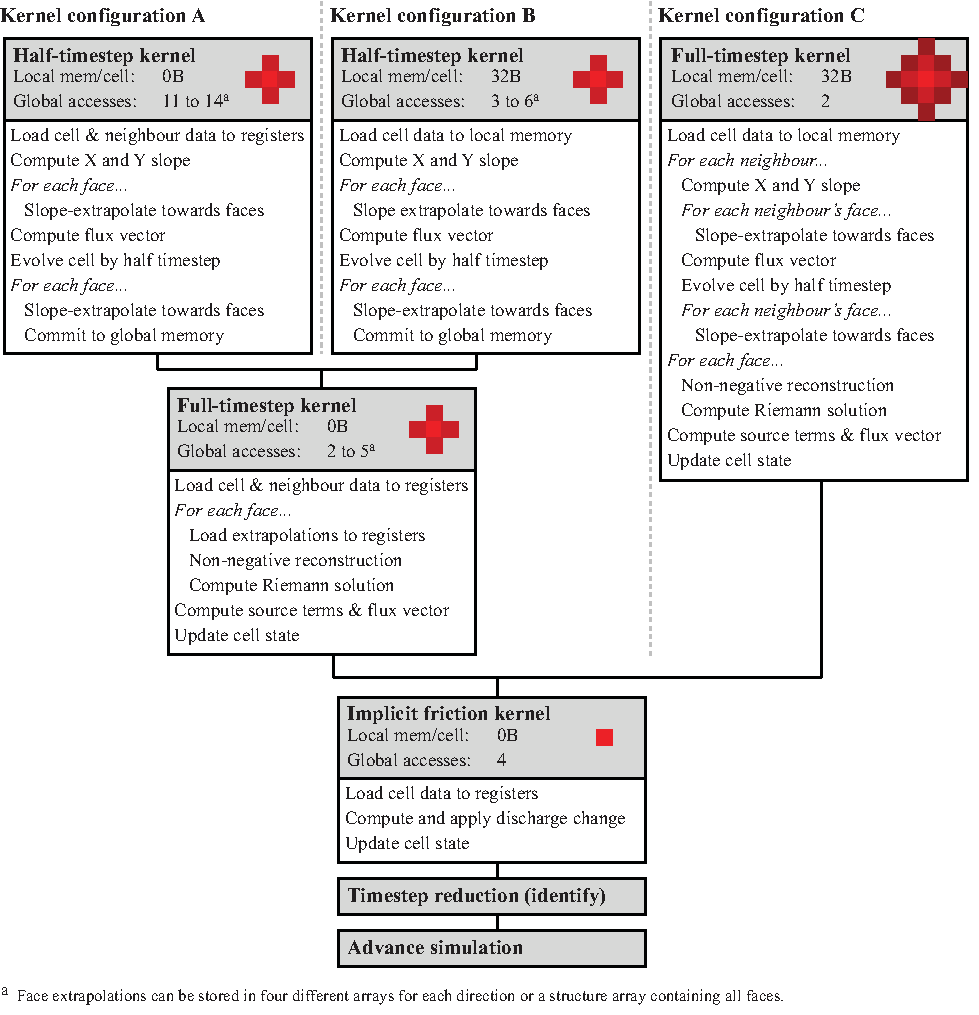
\includegraphics[width=1.0\textwidth]{heterogeneous-dev-figures/Figure_5_Colour.pdf}
	\caption{Implementation of the second-order MUSCL-Hancock scheme with three different kernel configurations intended to suit a majority of modern processing devices, and the data stencils for cell data required by each.}
	\label{Kernels}
\end{figure*}

To achieve high efficiency regardless of vendor differences, user-selectable kernel configurations are implemented to explore the effects of memory access patterns, illustrated in Figure \ref{Kernels} alongside the data stencils for each kernel. Configuration A is expected to perform well for devices with a high occupancy and sufficient resources to maintain enough warps/wavefronts to mask global memory latency, thus makes no use of local caching; configuration B introduces some caching to configuration A where possible in the half-timestep kernel, reducing the number of global accesses with irregular strides; and configuration C uses the maximum amount of caching and the least amount of global accesses, but the consequence is a greater computational burden because the half-timestep calculation must be repeated many times given that local memory is insufficiently sized to cache face extrapolated data. All high-end devices are expected to have enough resources (mainly registers) to perform best with configuration A. 

\section{User interface and platform availability}

\begin{figure*}[tpb]
	\centering
	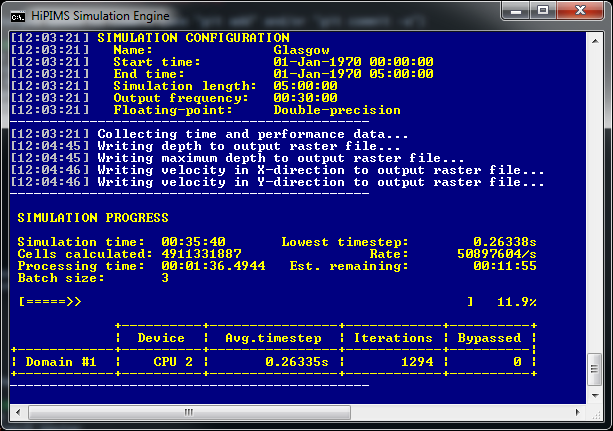
\includegraphics[width=0.9\textwidth]{software-figures/console-screenshot.png}
	\caption{Console-based version of the software, showing cell throughput on a CPU and the overall progress.}
	\label{Software_UI_Console}
\end{figure*}
\begin{figure*}[tpb]
	\centering
	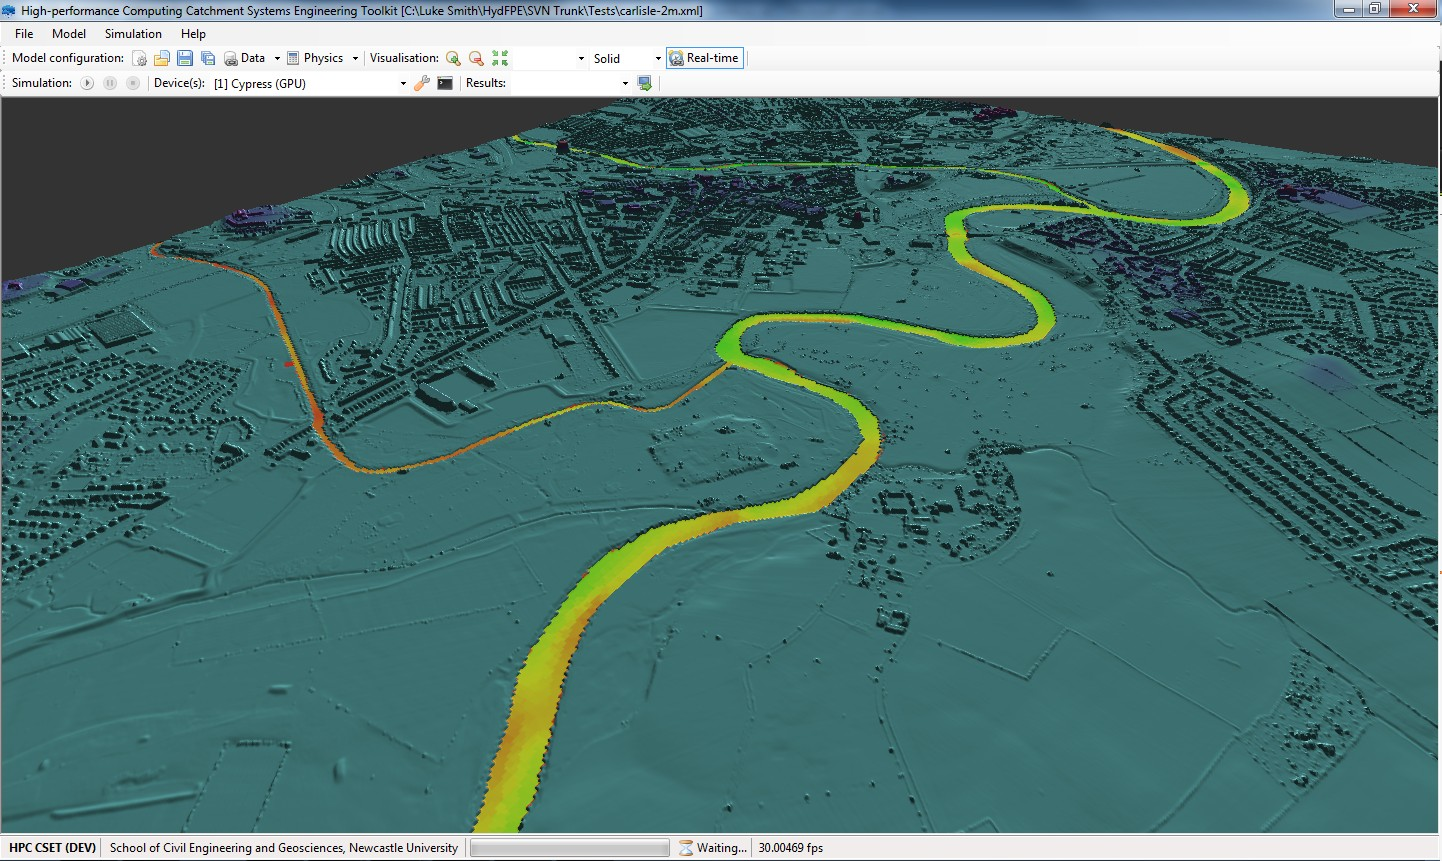
\includegraphics[width=1.0\textwidth]{software-figures/interface-screenshot.jpg}
	\caption{Windows-based version of the software, with real-time 3D visualisation of results, showing the initial state for a simulation of the Carlisle 2005 flood.}
	\label{Software_UI_3D}
\end{figure*}

Whilst non-contributory with respect to the fundamental research this thesis intends to provide, two user interfaces exist for the software. It is anticipated that the vast majority of applications for the software will be applied using high-performance computing servers, which are likely to only be accessible by console. A colour-enabled status console is provided, to report log messages, remaining time estimates, and overall simulation progress, as shown in Figure \ref{Software_UI_Console}. The software may be compiled for both Windows and Linux, for deployment to 32-bit and 64-bit architectures.

A more user-friendly interface already exists, capable of showing real-time simulation results in 3D, as in Figure \ref{Software_UI_3D}. A hue-based colour ramp is used to illustrate increasing depth. This interface uses a library-based version of the simulation engine, embedded within a C\# interface for consistency with other Windows applications, and OpenGL for 3D visualisation. Methods for improving the communication of simulation results are worthy of further research and discussion, but fall outside the scope of this thesis.

\section{Conclusions}

This chapter presented the numerical basis for a finite-volume solution to the shallow water equations, obtained using the HLLC method for approximately solving the Riemann problem, and thus creating a Godunov-type scheme. This is then extended to provide a second-order solution, by employing the MUSCL method. This computationally-intensive but versatile method is decomposed to stencil operations, such that each cell within the Cartesian domain is dependent only on a small number of neighbouring cells, and identification of the timestep from all cells in the domain is performed using a two-stage process which allows the processing to be shared across computing resources available. A number of different implementation patterns for the second-order solution allow caching to be leveraged, depending on the processing device employed.

The software described is capable of operating on CPU, GPU, and hybrid-style APU processing devices. The numerical and computational approach described is intended to make the software as versatile as possible, although there are nonetheless limitations to its applicability. The next chapter considers a wide range of flow scenarios and flood mechanisms, and evaluates the software's performance against each.